

\subsection{Program Template}

\code{src/template.cc}

\subsubsection{Compilation}
\begin{minted}{bash}
alias gg="g++ -std=gnu++20 -x c++ -Wall -O2 -static
-pipe -lm"
\end{minted}
{\color{gray}\texttt{(NWERC 2024)}}

\newpage

\subsection{Strategy}

\subsubsection{Solving strategy}
\begin{itemize}
    \item Go over all problems that haven't been solved.
    \item Small conditions $\rightarrow$ Brute force/less efficient algorithm.
    \item Do we need to take a break? Drink enough water!
    \item Should a solution be possible for \textit{all cases}? Think of special cases.
    \begin{itemize}
        \item Is it $<$ or $\leq$?
        \item Why would a special condition be given?
    \end{itemize}
    \item Sketch on paper.
    \item Did we read the problem correctly? Look at images on problem sheet.
    \item Use Python when working with very large numbers.
\end{itemize}

\subsubsection{Problem solving strategies}
\begin{itemize}
    \item \textbf{Greedy}: Pick best looking on each step.
    \item \textbf{Dynamic Programming}: Use table to remember results.
    \item \textbf{Backtracking}: Check intermediate results.
    \item \textbf{Divide and conquer}: Split up into smaller problems.
    \item \textbf{BFS/DFS/floodfill}.
    \item \textbf{Prefix/Suffix tree}: For string problems.
    \item \textbf{Create/Extend a graph}: Minimizing problems $\rightarrow$ use Dijkstra/Kruskal.
    \item \textbf{Hash table}: Up to around $10^8 \approx 2^{26.5}$ entries.
    \begin{itemize}
        \item Don't make too many hash tables!
    \end{itemize}
    \item \textbf{Matrix form}: Gain more insight in how parts interact.
    \item \textbf{Randomization}: Chance of failure is small enough.
    \item \textbf{Bitset}: Encode binary data. Useful for bitshifting.
    \item Use \textbf{polynomials} to model the problem.
    \item Consider the problem in \textbf{reverse}.
\end{itemize}

\subsubsection{Wrong answer}
\begin{itemize}
    \item Check boundary values: Minimum, maximum, powers of $2$.
    \item Division by $0$ $\rightarrow$ NaN.
    \item Off-by-one error?
    \item Is it $<$ or $\leq$?
    \item Input all $0$.
    \item Integer overflow or NaN.
    \item Can precision be influenced by transformation function? i.e. $\log$, $\exp$, etc.
    \item Does output have to be given modulo $M$?
\end{itemize}

\subsubsection{Timelimit}
\begin{itemize}
    \item Make sum/minimum calculation efficient.
    \item \texttt{DBG} statements can cause slowdowns.
    \item Use fast IO and flush output manually.
    \item Use hash tables or rolling hashes.
    \item Don't create too many sets or queues.
\end{itemize}

\subsubsection{Run error}
\begin{itemize}
    \item Forgot to compile?
    \item Check typos.
    \item Division by $0$?
    \item Accessing index $-1$ of vector?
\end{itemize}

\subsubsection{Memory limit}
\begin{itemize}
    \item Replace \texttt{long long} with \texttt{int}.
    \item Reduce DP table dimensions.
\end{itemize}



\subsection{Useful built-ins}

\code{src/cpp.cc}

\subsubsection{Python}
\code[python3]{src/py.py}





\section{Math}

\subsection{Factorization, multiples and primes}

\subsubsection{Greatest common denominator}
This algorithm uses the formula $\text{gcd}(a,b) = \text{gcd}(b,r)$ if $a = bq + r$, where $q \neq 0$, $r \geq 0$ are integers.
\code{src/math/gcd.cc}

The gcd also has the following properties:
\begin{align*}
    \text{gcd}(a, b, c) &= \text{gcd}(a, \text{gcd}(b, c)), \\
    \text{gcd}(a, b) &= \text{gcd}(b, a), \\
    \text{gcd}(a, 0) &= a.
\end{align*}

\subsubsection{Extended Euclidean algorithm}
We can also determine the (lowest) numbers that form the gcd with the following algorithm:
\code{src/math/euclidgcd.cc}

\subsubsection{Least common multiple}
\begin{align*}
    \text{lcm}(a, b) = \frac{|ab|}{\text{gcd}(a, b)}
\end{align*}

\subsubsection{Prime factorization $\mathcal O(\log n)$}
\code{src/math/fact.cc}

\subsubsection{Miller-Rabin primality test $\mathcal O(\log n)$}
This primality test works for $n < 2^{64}$. For the \texttt{modPower} function see the "Modular arithmetic" section.
\code{src/math/millerrabin.cc}

\subsubsection{Wilson's theorem}
A natural number $p > 1$ is a prime if and only if
\begin{align*}
    (p - 1)! \equiv -1 \mod p.
\end{align*}

\subsubsection{Euler totient function}
The Euler totient function $\varphi(n)$ returns the number of positive integers smaller than $n$ that are coprime with $n$. An algorithm to determine $\varphi(n)$ can be optimized by using the formula 
\begin{align*}
    \varphi(n) = n \prod_{p|n} \left(1 - \frac1p\right).
\end{align*}
\code{src/math/phi.cc}

\subsubsection{Sieve of Eratosthenes $\mathcal O(n\log(\log n))$}
This algorithm finds all primes lower than a number $n$, by keeping track of a table and marking multiples of primes as non-prime.
\code{src/math/erat.cc}

\subsubsection{Number of primes below $n$}
The number of primes $\pi(n)$ smaller than or equal to $n$ has the property
\begin{align*}
    \lim_{n \to \infty} \frac{\pi(n)\log n }{n} = 1.
\end{align*}



\subsection{Modular arithmetic}

\subsubsection{Basic properties}
\begin{align*}
    \left.\begin{array}{r}
        a_1 \equiv b_1 \mod n \\
        a_2 \equiv b_2 \mod n
    \end{array}\right\}
    \Rightarrow a_1a_2 \equiv b_1b_2 \mod n
\end{align*}
\begin{align*}
    \left.\begin{array}{r}
        a_1 \equiv b_1 \mod n \\
        a_2 \equiv b_2 \mod n
    \end{array}\right\}
    \Rightarrow a_1 + a_2 \equiv b_1 + b_2 \mod n
\end{align*}
\begin{align*}
    \left.\begin{array}{r}
        \text{gcd}(a, n) = 1 \\
        c \equiv d \mod \varphi(n)
    \end{array}\right\}
    \Rightarrow a^c \equiv a^d \mod n
\end{align*}

\subsubsection{Modulo multiplication $\mathcal O(\log y)$}
\code{src/math/modmul.cc}

\subsubsection{Modulo power $\mathcal O(\log p)$}
\code{src/math/modpow.cc}

\subsubsection{Equal modulo}
\code{src/math/modeq.cc}

\subsubsection{Chinese remainder theorem}
The Chinese remainder theorem states that for any $n, m > 1$ coprime and a number $x < nm$ there exist unique $a < n$ and $b < m$ such that
\begin{align*}
    x &\equiv a \mod n, \\
    x &\equiv b \mod m.
\end{align*}
The solution $x$ can be determined using the extended Euclidean algorithm.
\code{src/math/crt.cc}

\subsubsection{Inverse elements}
The inverse of an integer $a$ modulo $n$ can be found using the extended Euclidean algorithm. An inverse exists if and only if $\text{gcd}(a, n) = 1$. Likewise the system $a\cdot x \equiv b \mod n$ can be solved if $\text{gcd}(a, n)$ divides b.
\code{src/math/modsys.cc}



\subsection{Geometry}

\subsubsection{Area of a triangle}
\begin{align*}
    A = \sqrt{x(x - a)(x - b)(x - c)}
\end{align*}
where $a$, $b$ and $c$ are the side lengths and $x = (a + b + c)/2$.

\subsubsection{Area of a quadrilateral}
\begin{align*}
    A = \sqrt{(a-x)(b-x)(c-x)(d-x) - \cos^2\left(\frac{\theta_1 + \theta_2}2\right)}
\end{align*}
where $\theta_1$ and $\theta_2$ are opposing corners and $x = (a + b + c + d)/2$.

\subsubsection{Area of a simple polygon}
Given a simple polygon (no intersecting edges) with $n$ vertices $(x_0, y_0), (x_1, y_1), \dots, (x_n, y_n)$ where $(x_0, y_0) = (x_n, y_n)$. The area of the polygon is
\begin{align*}
    A = \frac12\left|\sum_{k=0}^{n-1} (x_ky_{k+1} - x_{k+1}y_k)\right|.
\end{align*}

\subsubsection{Area of a regular polyhedron}
Given the number of side edges $n$, and either the distance from the center to a vertex $r$ or the distance from the center to an edge $a$, the area of a regular polyhedron is
\begin{align*}
    A &= nr^2\sin\frac{\pi}{n}\cos\frac{\pi}{n} = a^2n\tan\frac{\pi}{n}.
\end{align*}

\subsubsection{Maximal quadrilateral problem}
The maximum area of a quadrilateral is given by $\sqrt{(a-x)(b-x)(c-x)(d-x)}$ where $x = (a + b + c + d)/2$. This way the opposing corners add up to $\pi$ and all points lie on a circle.

\subsubsection{Circles and spheres}
\begin{itemize}
    \item Circumference of a circle: $2\pi r$.
    \item Area of a circle: $\pi r^2$.
    \item Area of a $3$-D sphere: $4\pi r^2$.
\end{itemize}

\subsubsection{Circle-line intersection}
The intersection point(s) of a circle with center $(0, 0)$ and radius $r$, and a line given by points $(x_1, y_1)$ and $(x_2, y_3)$ are given by $(X_\pm, Y_\pm)$:
\begin{align*}
    d_x &= x_2 - x_1, \\
    d_y &= y_2 - y_1, \\
    d_r &= \sqrt{d_x^2 + d_y^2}, \\
    D &= x_1y_2 - x_2y_1, \\
    X_\pm &= \frac{Dd_y \pm \text{sgn}(d_y)d_x\sqrt{r^2d_r^2 - D^2}}{d_r^2}, \\
    Y_\pm &= \frac{-Dd_x \pm |d_y|\sqrt{r^2d_r^2 - D^2}}{d_r^2}.
\end{align*}
where $\text{sgn}(x)$ is $-1$ if $x < 0$ and $1$ otherwise.

\subsubsection{Circle-circle intersection}
The intersection point(s) of two circles with centers $(x_1, y_1)$ and $(x_2, y_2)$ and radii $r_1$ and $r_2$ are given by $(X_\pm, Y_\pm)$:
\begin{align*}
    d &= \sqrt{(x_1 - x_2)^2 + (y_1 - y_2)^2}, \\
    l &= \frac{r_1^2 - r_2^2 + d^2}{2d}, \\
    h &= \sqrt{r_1^2 - l^2}, \\
    X_\pm &= \frac ld(x_2 - x_1) \pm \frac hd (y_2 - y_1) + x_1, \\
    Y_\pm &= \frac ld(y_2 - y_1) \mp \frac hd(x_2 - x_1) + y_1.
\end{align*}

\subsubsection{Volume of an $n$-ball}
An $n$-ball with radius $r$ has the following volume:
\begin{align*}
    V_n(r) &= \left\{\begin{array}{ll}
        1, & \text{if }n = 0, \\
        2r, & \text{if }n = 1, \\
        \frac{2\pi}n r^2 V_{n-2}(r), & \text{if }n > 1. \\
    \end{array}\right.
\end{align*}

\subsubsection{Angle between two vectors}
Given two vectors $a, b \in \mathbb R^n$, the angle between them is given by
\begin{align*}
    \theta = \cos^{-1}\frac{a\cdot b}{||a||\cdot||b||}.
\end{align*}

\subsubsection{Distance from a point to a line}
Given line $\ell(t) = a + bt$ with $a, b \in \mathbb R^n$ and point $p \in \mathbb R^n$, the distance is
\begin{align*}
    d = \frac{(p - a) \times (p - b)}{||b - a||}.
\end{align*}
In $2$-D the line is given by $ax + by + c = 0$, then the distance to point $p = (x_p, y_p)$ is given by
\begin{align*}
    d = \frac{|ax_p + by_p + c|}{\sqrt{a^2 + b^2}}.
\end{align*}
Note that we can remove the absolute value to check if two points are on the same side of a line!

\subsubsection{Intersection of lines}
Let the lines $\ell_1$ and $\ell_2$ be given by the points $(x_1, y_1)$ and $(x_2, y_2)$ respectively $(x_3, y_3)$ and $(x_4, y_4)$. Then the $c = x, y$ coordinate of the intersection point $P$ is given by
\begin{align*}
    P_c &= \frac{(x_1y_2 - x_2y_1)(c_3 - c_4) - (c_1 - c_2)(x_3y_4 - x_4y_3)}{(x_1 - x_2)(y_3 - y_4) - (y_1 - y_2)(x_3 - x_4)}.
\end{align*}

\subsubsection{Angle sum property}
The sum of the angles on of an $n$-lateral is $\pi(n - 2)$. The sum of the exterior angles of a polygon is $2\pi$.

\subsubsection{Maximum points on a circle}
Given the angle $\alpha$, the maximum number of points on a circle is $M = \lfloor \frac{2\pi}\alpha\rfloor$. Given a minimum distance $d$ between the points:
\begin{align*}
    \alpha = 2 \sin^{-1} \frac d{2r}.
\end{align*}

\subsubsection{3-D shapes}
\begin{table}[H]
    \centering
    \begin{tabular}{|l|c|c|}
        \hline
        Shape & Area & Volume \\
        \hline
        Cylinder & $2\pi rh + 2\pi r^2$ & $\pi r^2 h$ \\
        Cone & $\pi r\sqrt{r^2+h^2} + \pi r^2$ & $\frac13 \pi r^2 h$ \\
        \makecell[l]{Hemisphere\\(half sphere)} & $3\pi r^2$ & $\frac23\pi r^3$ \\
        Pyramid & \makecell{$lw + l\sqrt{\frac{w^2}4 + h^2}$\\$+ \sqrt{\frac{l^2}4 + h^2}$} & $\frac13lwh$ \\
        Torus & $4\pi^2Rr$ & $2\pi^2Rr^2$ \\
        Tetrahedron & $\sqrt3 a^2$ & $\frac{\sqrt2}{12}a^3$ \\
        Octahedron & $2\sqrt3 a^2$ & $\frac{\sqrt2}3 a^3$ \\
        Dodecahedron & $3\sqrt{25 + 10\sqrt5}a^2$ & $\frac14(15 + 7\sqrt5)a^3$ \\
        \hline
    \end{tabular}
    \label{tab:shapes}
\end{table}

\subsubsection{Distance on a sphere}
Given latitudes $\varphi_1, \varphi_2 \in [-\frac\pi2, \frac\pi2]$ and longitudes $\lambda_1, \lambda_2 \in [-\pi, \pi]$ the distance "as the crow flies" on a sphere with radius $R > 0$ between $(\varphi_1, \lambda_1)$ and $(\varphi_2, \lambda_2)$ is given by $d$:
\begin{align*}
    a &= \sin^2\frac{\varphi_2 - \varphi_1}2 + \cos\varphi_1 \cos\varphi_2 \sin^2\frac{\lambda_2 - \lambda_1}2, \\
    c &= 2\cdot\text{atan2}(\sqrt a, \sqrt{1 - a}), \\
    d &= Rc.
\end{align*}
The function $\text{atan2}$ is available in \texttt{C++} STL.

% \subsubsection{Diagonals of a polygon}
% The number of diagonals of an $n$-sided polygon is $\frac12n(n - 3)$.

\subsubsection{Weighted average of triangle vertices}
Given a (proper) triangle in $2$-D space with vertices $v_1, v_2, v_3 \in \mathbb R^2$ and a point $p \in \mathbb R^2$ inside the triangle. The following calculates weights $w_1, w_2, w_3 \in [0, 1]$ such that $p = w_1v_1 + w_2v_2 + w_3v_3$ with $w_1 + w_2 + w_3 = 1$.

Note that this implementation uses the "Distance from a point to a line" formula.
\code{src/math/triangleweight.cc}

\subsubsection{Convex hull $\mathcal O(n \log n)$}
The convex hull of a set $A$ is defined as
\begin{align*}
    \text{conv}(A) = \{\lambda x + (1 - \lambda) y \mid x, y \in A, \lambda \in [0, 1]\}.
\end{align*}
Given a finite set of points, their convex hull is a convex polygon with vertices that are in the original set of points. Using the Graham scan algorithm this subset of points can be determined.
\code{src/math/convexhull.cc}



\subsection{Useful numbers}

\begin{itemize}
    \item Prime numbers: $31$, $1031$, $32771$, $1048583$, $8125343$, $33554467$, $9982451653$, $1073741827$, $34359738421$, $1099511627791$, $35184372088891$, $1125899906842679$, $36028797018963971$, $10^3 + \{-9,-3,9,13\}$, $10^6 + \{-17,3,33\}$, $10^9 + \{7,9,21,33,87\}$.
    \item $\pi = \cos^{-1}(-1) = 3.14159265358979323846264\dots$.
    \item $\varphi = \frac{1 + \sqrt5}{2}$.
    \item $\log_{10}(2^{32}) \approx 9.632$, $\log_{10}(2^{64}) \approx 19.266$, $10^9 \approx 2^{30}$.
    \item Fibonacci numbers: $F_{n+2} = F_{n+1} + F_n$, starts with $0$, $1$. Lucas numbers start with $2$, $1$.
    \begin{itemize}
        \item $\lim_{n \to \infty} \frac{F_{n+1}}{F_n} = \lim_{n \to \infty} \frac{L_{n+1}}{L_n} = \varphi$.
        \item $F_{n-1}F_{n+1} - F_n^2 = (-1)^n$.
        \item $F_{n+k} = F_kF_{n+1} + F_{k-1}F_n$.
    \end{itemize}
    \item Catalan numbers: $C_n = \frac1{n + 1}\binom{2n}n$, $C_0 = 1$.
    \begin{itemize}
        \item $C_{n+1} = \sum_{k=0}^n C_kC_{n-k}$.
        \item $C_{n+1} = \frac{4n + 2}{n + 2}C_n$
    \end{itemize}
\end{itemize}

\subsubsection{Modular inverses}
\begin{table}[H]
    \centering
    \begin{tabular}{|c|c|c|}
        \hline
        $p$ & $M$ & $p^{-1} \mod M$ \\
        \hline
        $31$ & $33554467$ & $6494413$ \\
        $1031$ & $33554467$ & $28802816$ \\
        $32771$ & $33554467$ & $24638282$ \\
        $8125343$ & $33554467$ & $14214340$ \\
        $31$ & $36028797018963971$ & $26731042949553914$ \\
        $1031$ & $36028797018963971$ & $11776629093492588$ \\
        $32771$ & $36028797018963971$ & $30736232591595488$ \\
        $8125343$ & $36028797018963971$ & $34789068517540942$ \\
        \hline
    \end{tabular}
    \label{tab:modinv}
\end{table}



\subsection{Matrices}

\subsubsection{Gaussian elimination $\mathcal O(nm\min\{n,m\})$}
Gaussian elimination is used to reduce a matrix to reduced row echelon form. This form is useful for calculating the determinant, finding the inverse, etc.
\code{src/math/gauss.cc}

\subsubsection{Determinant of a matrix $\mathcal{O}(n^3)$}
Defined recursively as $|A| = a_{11}$ if $A \in \text{Mat}(1 \times 1)$, and
for \textit{any} $j$ and $A \in \text{Mat}(n \times n)$:
\begin{align*}
    |A| := \sum_{i=1}^n (-1)^{i+j} a_{ij} \cdot |\tilde A_{ij}|.
\end{align*}
where $\tilde A_{ij}$ is the matrix $A$ with row $i$ and column $j$ removed. The determinant can be determined more quickly by reducing the matrix to reduced row-echelon form and keeping track of row multiplications (see above).

\subsubsection{Multiplying two matrices $\mathcal O(Nnm)$}
Multiplication of matrices $A \in \text{Mat}(n \times N)$ and $B \in \text{Mat}(N \times m)$ is defined as
\begin{align*}
    (AB)_{ij} &= \sum_{k=1}^N A_{ik} B_{kj}
\end{align*}
so that $AB \in \text{Mat}(n \times m)$.
% \code{src/math/matmul.cc}

\subsubsection{Inverse of a matrix $\mathcal O(n^3)$}
The inverse of a matrix can be determined with the formula
\begin{align*}
    A^{-1} = \frac1{|A|}\text{adj}(A),
\end{align*}
where $(\text{adj}(A))_{ij} := (-1)^{i + j}C_{ji}$ with $C_{ji}$ the determinant of $A$ with row $j$ and column $i$ removed. This makes it possible to determine the inverse without division, but is $\mathcal O(n^5)$. The following implementation uses Gaussian elimination, which is $\mathcal O(n^3)$.
\code{src/math/matinv.cc}

\subsubsection{Miscellaneous}
\begin{itemize}
    \item $\left|\begin{array}{cc}A & B \\ 0 & D\end{array}\right| = |A|\cdot|D|$.
    \item If $A$ is invertable, then $\left|\begin{array}{cc}A & B \\ C & D\end{array}\right| = |A|\cdot|D - CA^{-1}B|$.
    \item For $A, B \in \text{Mat}(n \times n)$, $\left|\begin{array}{cc}A & B \\ B & A\end{array}\right| = |A - B|\cdot|A + B|$.
    \item For $A, B \in \text{Mat}(2 \times 2)$, $|A + B| = |A| + |B| + \text{tr}(A)\text{tr}(B) - \text{tr}(AB)$.
    \item $|A + B| \geq |A| + |B|$.
    \item $|cA| = c^n|A|$.
    \item $|A^\top| = |A|$.
    \item $|AB| = |A|\cdot|B|$.
    \item $|A^{-1}| = |A|^{-1}$.
    \item $|A| = \prod_{i=1}^n \lambda_i$.
    \item $\frac n{\text{tr}(A^{-1})} \leq |A|^{1/n} \leq \frac1n\text{tr}(A)$.
    \item $\left(\begin{array}{cc}a & b \\ c & d\end{array}\right)^{-1} = \frac1{ad - bc}\left(\begin{array}{cc}d & -b \\ -c & a\end{array}\right)$.
    \item $\text{tr}(A) := \sum_{i=1}^n a_i$.
    \item For $A, B \in \text{Mat}(n \times m)$ we have $\text{tr}(A^\top B) = \text{tr}(AB^\top) = \text{tr}(B^\top A) = \text{tr}(BA^\top) = \sum_{i=1}^m\sum_{j=1}^n a_{ij}b_{ij}$.
    \item $\text{tr}(ABCD) = \text{tr}(BCDA)$.
    \item $\text{tr}(P^{-1}AP) = \text{tr}(A)$.
    \item $\text{tr}(A) = \sum_{i=1}^n \lambda_i$.
\end{itemize}



\subsection{Linear equation solver $\mathcal O(nm\min\{n, m\})$}

\code{src/math/linsys.cc}



\subsection{Roots of polynomials}

\subsubsection{Linear}
The system $ax + b = 0$ has one solution if $a \neq 0$, given by
\begin{align*}
    x = - \frac ba.
\end{align*}

\subsubsection{Quadratic}
The system $ax^2 + bx + c = 0$ has at most two (possibly complex) solutions if $a \neq 0$, given by
\begin{align*}
    x_\pm = \frac{-b \pm \sqrt{b^2 - 4ac}}{2a}.
\end{align*}

\subsubsection{Cubic}
Given is a cubic equation $ax^3 + bx^2 + cx + d = 0$ with $a \neq 0$. Define
\begin{align*}
    \Delta_0 &= b^2 - 3ac, \\
    \Delta_1 &= 2b^3 - 9abc + 27a^2d, \\
    C &= \sqrt[3]{\frac{\Delta_1 \pm \sqrt{\Delta_1^2 - 4\Delta_0^3}}2}, \\
    \xi &= \frac{-1 + \sqrt{-3}}2.
\end{align*}
In the case of a complex number, any square root or cube root in the formula for $C$ can be taken (there are multiple). The sign in the formula for $C$ should be chosen such that $C \neq 0$. The three solutions are given by
\begin{align*}
    x_k = -\frac1{3a}\left(b + \xi^kC + \frac{\Delta_0}{\xi^k C}\right), \qquad k \in \{0, 1, 2\}.
\end{align*}





\subsection{Series and sums}

\begin{itemize}
    \item Zeta constants: $\zeta(2n) = \sum_{k=1}^\infty \frac1{k^{2n}}$.
    \begin{itemize}
        \item $\zeta(2) = \sum_{n=1}^\infty \frac1{n^2} = \frac{\pi^2}6$.
        \item $\zeta(4) = \sum_{n=1}^\infty \frac1{n^4} = \frac{\pi^4}{90}$.
        \item $\zeta(6) = \sum_{n=1}^\infty \frac1{n^6} = \frac{\pi^6}{945}$.
    \end{itemize}
    \item $\sum_{k=1}^m k = \frac{m(m+1)}2$.
    \item $\sum_{k=1}^m k^2 = \frac{m(m+1)(2m + 1)} 6 = \frac{m^3}3 + \frac{m^2}2 + \frac m6$.
    \item $\sum_{k=1}^m k^3 = \left(\frac{m(m+1)}2\right)^2 = \frac{m^4}4 + \frac{m^3}2 + \frac{m^2}4$.
    \item $\sum_{k=m}^n z^k = \frac{z^m - z^{n+1}}{1 - z}$.
    \item Polylogarithm:
    \begin{itemize}
        \item $\sum_{k=1}^\infty \frac{z^k}k = -\ln(1 - z)$.
        \item $\sum_{k=1}^\infty z^k = \frac z{1 - z}$.
        \item $\sum_{k=1}^\infty kz^k = \frac z{(1 - z)^2}$.
        \item $\sum_{k=1}^\infty k^2z^k = \frac {z(1 + z)}{(1 - z)^3}$.
    \end{itemize}
    \item Exponential function:
    \begin{itemize}
        \item $\sum_{k=0}^\infty \frac{z^k}{k!} = e^z$.
        \item $\sum_{k=0}^\infty k\frac{z^k}{k!} = ze^z$.
        \item $\sum_{k=0}^\infty k^2\frac{z^k}{k!} = (z + z^2)e^z$.
    \end{itemize}
    \item Trigonometry:
    \begin{itemize}
        \item $\sin z = \sum_{k=0}^\infty \frac{(-1)^k z^{2k + 1}}{(2k + 1)!}$.
        \item $\sinh z = \sum_{k=0}^\infty \frac{z^{2k + 1}}{(2k + 1)!}$.
        \item $\cos z = \sum_{k=0}^\infty \frac{(-1)^k z^{2k}}{(2k)!}$.
        \item $\cosh z = \sum_{k=0}^\infty \frac{z^{2k}}{(2k)!}$.
    \end{itemize}
    \item Binomial coefficients:
    \begin{itemize}
        \item $\sum_{k=0}^n \binom nk = 2^n$.
        \item $\sum_{k=0}^n (-1)^k \binom nk = 0$ for $n \geq 1$.
        \item $\sum_{k=0}^n \binom km = \binom{n+1}{m+1}$.
        \item $\sum_{k=0}^n \binom{m + k - 1}{k} = \binom{n + m}{n}$.
        \item $\sum_{k=0}^n \binom\alpha k \binom\beta{n - k} = \binom{\alpha + \beta}{n}$.
    \end{itemize}
    \item $\sum_{k=1}^\infty \frac{(-1)^{k+1}}k = \log2$.
    \item $\sum_{k=1}^\infty \frac{(-1)^{k+1}}{2k - 1} = \frac\pi4$.
\end{itemize}

\subsubsection{Minimum squared difference}
\begin{align*}
    \argmin_{x \in \mathbb R} \sum_{k=1}^n (x_k - x)^2 = \frac1n\sum_{k=1}^n x_k
\end{align*}

\subsubsection{Binomials $\mathcal O(n)$}
The binomial "$n$ choose $k$" (typically $k \leq n$) is defined as
\begin{align*}
    \binom nk = \frac{n!}{k!(n - k)!}.
\end{align*}
Then Newton's binomial theorem says that for $z \in \mathbb C$, $|z| < 1$ and $r \geq 0$ we have
\begin{align*}
    (1 + z)^r = \sum_{k=0}^\infty \binom rk z^k
\end{align*}
Calculating a high power of a sum of $x, y \in \mathbb C$ is done with
\begin{align*}
    (x + y)^n = \sum_{k=0}^n \binom nk x^{n-k}y^k.
\end{align*}
\code{src/math/binom.cc}



\subsection{Probability}

\subsubsection{Basic properties}
\begin{itemize}
    \item $\mathbb E[X] = \sum_{x \in \Omega} x\mathbb P(X = x)$.
    \item $\mathbb E[X] = \mathbb E[X \mid A]\mathbb P(X \in A) + \mathbb E[X \mid B]\mathbb P(X \in B)$, when $\Omega = A \cup B$ and $A \cap B = \varnothing$.
    \item $\mathbb E[aX + bY] = a\mathbb E[X] + b\mathbb E[Y]$.
    \item $\mathbb P(X \in A) = 1 - \mathbb P(X \not\in A)$.
    \item $\mathbb P(X \leq x) = \mathbb P(X = x) + \mathbb P(X < x)$.
    \item $\mathbb P(X \in A) = \mathbb P(X \in A_1) + \mathbb P(X \in A_2)$, when $A = A_1 \cup A_2$ and $A_1 \cap A_2 = \varnothing$.
    \item $\mathbb P(X \mid Y) = \mathbb P(X \cap Y) / \mathbb P(Y)$.
\end{itemize}

\subsubsection{Bayes' Theorem}
\begin{align*}
    \mathbb P(X \mid Y) = \frac{\mathbb P(Y \mid X)P(X)}{P(Y)}
\end{align*}

\subsubsection{Independence}
Two random variables $X$ and $Y$ are independent if $\mathbb P(X \cap Y) = \mathbb P(X)\mathbb P(Y)$.

When random variables $X_1, \dots, X_n$ are independent and identically distributed, we have
\begin{align*}
    \mathbb P(X_1 = \dots = X_n = x) = \mathbb P(X_1 = x)^n.
\end{align*}

\subsubsection{Hölder's inequality}
For $p, q \in [1, \infty)$ with $\frac1p + \frac1q = 1$ and $f, g$ $\mu$-measurable ("normal" functions) we have
\begin{align*}
    \int |fg|\ d\mu \leq \left(\int |f|^p\ d\mu\right)^{\frac1p}\left(\int |g|^q\ d\mu\right)^{\frac1q}.
\end{align*}

\subsubsection{Markov Chains}
A Markov chain is given by a transition matrix, which gives to probability to transition from one state to another:
\begin{align*}
    P_{ij} = \mathbb P(X_n = j \mid X_{n-1} = i).
\end{align*}
In particular Markov chains have the Markov property:
\begin{align*}
    &\quad\ \mathbb P(X_{n+1} = x \mid X_1 = x_1, \dots, X_n = x_n) \\
    &= \mathbb P(X_{n+1} = x \mid X_n = x_n).
\end{align*}
Suppose that we have a Markov chain with matrix
\begin{align*}
    P = \left(\begin{array}{cc}
        Q & R \\
        0 & I_r
    \end{array}\right).
\end{align*}
This Markov chain is absorbing, with $r$ absorbing states (and $t$ transient states). The fundamental matrix is defined as
\begin{align*}
    N = (I_t - Q)^{-1}.
\end{align*}
Then the expected number of steps before being absorbed, starting in state $i$, is the $i$-th entry in the vector $N\mathbbm 1$. The probability of being absorbed into absorbing state $j$, starting from state $i$, is the $i,j$-entry in $NR$.

The probability of visiting transient state $j$ when starting in transient state $i$ is the $i,j$-entry in $(N - I_t)(N_{\text{dg}})^{-1}$. Here $N_{\text{dg}}$ is the diagonal matrix with the same diagonal as $N$.

\subsubsection{Common distributions}
Distributions below are over some discrete set (support).
\begin{table}[H]
    \centering
    \begin{tabular}{|l|c|c|c|c|}
        \hline
        Name & $\mathbb P(X = k)$ & Supp. & $\mu$ & $\sigma^2$ \\
        \hline
        Bern. & $p^{1-k}(1-p)^k$ & $\{0, 1\}$ & $p$ & $p(1 - p)$ \\
        Bin. & $\binom nk p^k(1-p)^{n-k}$ & $\{0, \dots, n\}$ & $np$ & $np(1-p)$ \\
        Geo. & $(1 - p)^{k-1}p$ & $\mathbb N_0$ & $\frac1p$ & $\frac{1-p}{p^2}$ \\
        Pois. & $\frac{\lambda^ke^{-\lambda}}{k!}$ & $\mathbb N_0$ & $\lambda$ & $\lambda$ \\
        Unif. & $\frac1{b-a+1}$ & $\{a, \dots, b\}$ & $\frac{a + b}2$ & $\frac{(b - a + 1)^2 - 1}{12}$ \\
        \hline
    \end{tabular}
    \label{tab:distr_discrete}
\end{table}
Distributions below are over some continuous set (support), given are density functions $f$.
\begin{table}[H]
    \centering
    \begin{tabular}{|l|c|c|c|c|}
        \hline
        Name & $f(x)$ & Supp. & $\mu$ & $\sigma^2$ \\
        \hline
        Beta & $\frac{x^{\alpha-1}(1 - x)^{\beta-1}}{B(\alpha, \beta)}$ & $[0, 1]$ & $\frac\alpha{\alpha+\beta}$ & $\frac{\alpha\beta}{(\alpha+\beta)^2(\alpha+\beta+1)}$ \\
        Unif. & $\frac1{b-a}$ & $[a, b]$ & $\frac{a + b}2$ & $\frac{(b-a)^2}{12}$ \\
        Exp. & $\lambda e^{-\lambda x}$ & $[0, \infty)$ & $\frac1\lambda$ & $\frac1{\lambda^2}$ \\
        Gam. & $\frac{x^{k-1}e^{-x/\theta}}{\Gamma(k)\theta^k}$ & $(0, \infty)$ & $k\theta$ & $k\theta^2$ \\
        Nor. & $\frac{\exp\left(-\frac{(x-\mu)^2}{(\sigma^2}\right)}{\sigma\sqrt{2\pi}}$ & $\mathbb R$ & $\mu$ & $\sigma^2$ \\
        $t$, $\nu = 1$ & $\frac1{\pi(1+t^2)}$ & $\mathbb R$ & & \\
        \hline
    \end{tabular}
    \label{tab:distr_cont}
\end{table}
The beta and gamma functions are defined as
\begin{align*}
    B(\alpha, \beta) &= \int_0^1 t^{\alpha-1}(1-t)^{\beta-1}\ dt, \\
    \Gamma(k) &= (k - 1)! = \int_0^\infty t^{k-1}e^{-t}\ dt.
\end{align*}

\subsubsection{Common situations}
\begin{itemize}
    \item Suppose an event happens event time unit with probability $p$, then the probability of having it occur \textit{exactly} $n$ times in the first $m$ time units ($m \geq n$) is equal to
    \begin{align*}
        \mathbb P(S = n) = \binom{m}{n} p^{n}(1-p)^{m-n}.
    \end{align*}
    The probability of it happening \textit{at least} $n$ times is then
    \begin{align*}
        \mathbb P(S \geq n) = \sum_{k=n}^m \mathbb P(S = k).
    \end{align*}
    \item Given a game with $n$ rounds, where the prizes making it through to round $i$ are $r_i$ and the probability of making it through round $i$ is $p_i$. The player can stop at any round (including before the first round). Then the expected winnings $W$ playing optimally, given that the player is currently at round $I$ are
    \begin{align*}
        \mathbb E[W \mid I = i] &= \max\left\{r_i,\ p_i\mathbb E[W \mid I = i + 1]\right\}, \\
        \mathbb E[W] &= \mathbb E[W \mid I = 0].
    \end{align*}
    \item Assume we grab items from a set without putting them back, until there are no more items left. If each item is chosen with the same probability, then the probability of a specific sequence is
    \begin{align*}
        \mathbb P(X_1 = x_1, \dots, X_n = x_n) = \frac1{n!}.
    \end{align*}
    \item Usually DP is very useful for probability problems.
\end{itemize}

\subsubsection{Entropy}

Entropy indicates the uncertainty factor of a random variable. The definition of entropy is
\begin{align*}
    H(X) = -\sum_{x\in\mathcal X}p(x)\log_2 p(x) = \mathbb E[-\log_2 p(X)].
\end{align*}
Some properties are:
\begin{itemize}
    \item For any function $f$, $H(f(X)) \leq H(X)$.
    \item For $X$ and $Y$ independent, $H(X\mid Y) = H(X)$.
    \item For any $X$ and $Y$, $H(X\mid Y) \leq H(X)$.
    \item For any $X$ and $Y$, $H(Y, X) = H(X,Y) = H(X\mid Y) + H(Y)$.
\end{itemize}



\subsection{Combinatorics}

\subsubsection{Burnside's lemma}
Let $G$ be a finite group that acts on a set $X$, let $X^g$ be the set of elements in $X$ that are fixed by $g$, then the number of orbits is
\begin{align*}
    |X / G| = \frac1{|G|}\sum_{g \in G} |X^g|.
\end{align*}

\subsubsection{Pólya enumeration theorem (unweighted)}
Let $G$ be a group of permutations of a finite set $X$. Denote $Y^X$ for all functions $X \to Y$. Then the group $G$ acts on $Y^X$, and the number of orbits is
\begin{align*}
    |Y^X / G| = \frac1{|G|}\sum_{g \in G} |Y|^{c(g)},
\end{align*}
where $c(g)$ is the number of cycles of $g$ when viewed as a permutation of $X$.

\subsubsection{$k$-th combination $\mathcal O(n\log n)$}
Given a number $n$, the following returns the $k$-th combination in the list of bit sequences of length $n$ that contain $m$ ones. Note that the total number of combinations is $\binom nm$.
\code{src/math/nthcomb.cc}

\subsubsection{List of combinations $\mathcal O(n\binom nm)$}
Given numbers $n$ and $m$, the following produces a list of all bit sequences of length $n$ that contain $m$ ones, without enumerating over all $2^n$ possible bit sequences of length $n$.
\code{src/math/allcombs.cc}



\subsection{Analysis and calculus}

% \subsubsection{Integral definition}
% For any piece-wise continuous $f$, the integral of $f$ on $[a, b]$ is defined as
% \begin{align*}
%     \int_a^b f(x)\ dx = \lim_{n \to \infty} \frac{b - a}n \sum_{k=0}^{n-1} f\left(a + k\frac{b - a}n\right).
% \end{align*}

% \subsubsection{Derivative definition}
% Assuming the limit exists, the derivative of $f$ is defined as
% \begin{align*}
%     f'(x) = \lim_{h \to 0} \frac{f(x + h) - f(x)}h.
% \end{align*}

\subsubsection{L'Hôpital's rule}
If $\lim_{x\to c} f(x) = \lim_{x \to c} g(x) = 0$ and the right limit exists, then
\begin{align*}
    \lim_{x \to c} \frac{f(x)}{g(x)} = \lim_{x \to c} \frac{f'(x)}{g'(x)}.
\end{align*}

\subsubsection{Integration by parts}
\begin{align*}
    \int_a^b f'(x)g(x)\ dx = \left[f(x)g(x)\right]_a^b - \int_a^b f(x)g'(x)\ dx.
\end{align*}

\subsubsection{Common integrals}
\begin{align*}
    \int \tan x\ dx = -\log|\cos x| + C
\end{align*}
\begin{align*}
    \int \cot x\ dx = \log|\sin x| + C
\end{align*}
\begin{align*}
    \int \csc x\ dx = \log|\csc x + \cot x| + C
\end{align*}
\begin{align*}
    \int \sec x\ dx = \log|\sec x + \tan x| + C
\end{align*}
\begin{align*}
    \int_0^\infty e^{-ax^2}\ dx = \frac12\sqrt{\frac \pi a}
\end{align*}
\begin{align*}
    \int_0^\infty \frac x{e^x - 1}\ dx = \frac{\pi^2}6
\end{align*}

\subsubsection{Common derivatives}
\begin{align*}
    \frac{d}{dx}\sin^{-1}x = \frac1{\sqrt{1-x^2}}
\end{align*}
\begin{align*}
    \frac{d}{dx}\cos^{-1}x = -\frac1{\sqrt{1-x^2}}
\end{align*}
\begin{align*}
    \frac{d}{dx}\tan^{-1}x = \frac1{1+x^2}
\end{align*}

\subsubsection{Common limits}
\begin{align*}
    \lim_{x \to 0}\frac{a^x - 1}x = \log a
\end{align*}
\begin{align*}
    \lim_{x \to 0} \frac{\sin(ax)}{bx} = \frac ab, \qquad \text{if }b \neq 0
\end{align*}
\begin{align*}
    \lim_{n \to \infty} \frac n{\sqrt[n]{n!}} = e
\end{align*}
\begin{align*}
    \lim_{n \to \infty} \frac{\sqrt{2\pi n}\left(\frac ne\right)^n}{n!} = 1, \qquad \text{(Stirling)}
\end{align*}

\subsubsection{Partial fractions}
A fraction with a product of linear expressions at the bottom can be split:
\begin{align*}
    \frac{ax + b}{(x - a_1)\dots(x - a_m)} = \frac{A_1}{x - a_1} + \dots + \frac{A_2}{x - a_m}.
\end{align*}
Find the $A_i$ by solving the system of equations that you get when transforming the sum into one fraction and comparing the factors before $x$ and the constants.

\subsubsection{Newton's method}
For most differentiable functions $f$ and sequences $(x_n)_{n=0}^\infty$ with
\begin{align*}
    x_{n + 1} = x_n - \frac{f(x_n)}{f'(x_n)},
\end{align*}
the sequence $(f(x_n))_{n=0}^\infty$ will converge to zero, i.e. the limit of $(x_n)_{n=0}^\infty$ is a root of $f$. Newton's method uses this property to find roots of functions, by starting with $x_0$ close to a root.
\code{src/math/newton.cc}

\subsubsection{Extremum of a parabola}
The minimum or maximum of a parabola with the formula $y = ax^2 + bx + c$ is given by the point
\begin{align*}
    (x, y) &= \left(-\frac b{2a}, c - \frac{b^2}{4a}\right).
\end{align*}



\subsection{Fast Fourier transform $\mathcal O(n\log n)$}

The discrete Fourier transform of the polynomial $A(x) = a_0x^0 + \dots + a_{n - 1}x^{n - 1}$ with $n = 2^m$ is defined as
\begin{align*}
    \mathcal F(a_0, \dots, a_{n - 1}) = (A(w_n^0), \dots, A(w_n^{n-1})),
\end{align*}
where $w_n = \exp(\frac{2\pi i}n)$. When multiplying polynomials $A$ and $B$ we have $\mathcal F(A\cdot B) = \mathcal F(A) \cdot\mathcal F(B)$ where multiplication is done coordinate-wise. This gives
\begin{align*}
    A\cdot B = \mathcal F^{-1}(\mathcal F(A)\cdot \mathcal F(B)).
\end{align*}
FFT can also be used to multiply two very large numbers quickly, by using the multiplication of polynomials and filling in $x = 10$.

\code{src/math/fft.cc}





\section{Data structures}

\code{src/datastr/builtin.cc}

\subsection{Disjoint-set union}

The disjoint-set structure is used to represent a partition of dataset. It supports two basic operations:
\begin{itemize}
    \item \textsc{find:} Returns the representative of the subset that the given item is a part of. The representative is the same for any item in the same subset. $\mathcal O(\alpha(n))$
    \item \textsc{combine:} (union) Combine two subsets, making the representatives of the items in the set the same. $\mathcal O(\alpha(n))$
\end{itemize}
\begin{figure}[H]
    \centering
    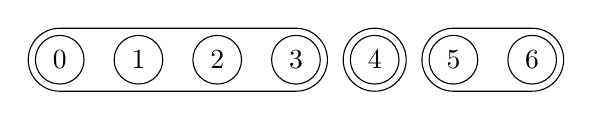
\begin{tikzpicture}
        \draw[rounded corners=0.4cm, draw=black] (-1.4, -0.4) rectangle (2.4, 0.4);
        \draw[rounded corners=0.4cm, draw=black] (2.6, -0.4) rectangle (3.4, 0.4);
        \draw[rounded corners=0.4cm, draw=black] (3.6, -0.4) rectangle (5.4, 0.4);
        \node[draw, circle] at (-1, 0) (0) {$0$};
        \node[draw, circle] at (0, 0) (0) {$1$};
        \node[draw, circle] at (1, 0) (0) {$2$};
        \node[draw, circle] at (2, 0) (0) {$3$};
        \node[draw, circle] at (3, 0) (0) {$4$};
        \node[draw, circle] at (4, 0) (0) {$5$};
        \node[draw, circle] at (5, 0) (0) {$6$};
    \end{tikzpicture}
\end{figure}
\vspace{-0.3cm}
The implementation uses a list of numbers $\{0, \dots, n - 1\}$. These can then be used as indices of more complex data. The unions are represented as rooted trees, where every node points to its representative. The $\alpha$ in the complexities above is a very slow growing function. The implementation below is an expanded version of the basic DSU data structure.
\code{src/datastr/dsu.cc}



\subsection{Trie}

A trie is used to represent a collection of strings. It stores the prefixes of strings in a tree structure. For example the strings  \texttt{aab}, \texttt{aabc} and \texttt{aacb} are represented as:
\vspace{-0.3cm}
\begin{figure}[H]
    \centering
    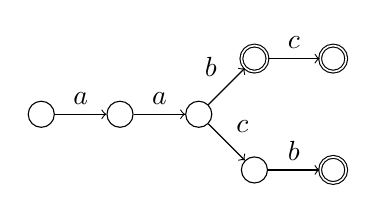
\begin{tikzpicture}[main/.style = {draw, circle}, node distance=1cm]
        \node[main] (0) {};
        \node[main] (1) [right of=0] {};
        \node[main] (2) [right of=1] {};
        \node[main,double] (3) [above right of=2] {};
        \node[main,double] (4) [right of=3] {};
        \node[main] (5) [below right of=2] {};
        \node[main,double] (6) [right of=5] {};
        \draw[->] (0) -- node[midway, above] {$a$} (1);
        \draw[->] (1) -- node[midway, above] {$a$} (2);
        \draw[->] (2) -- node[midway, above left] {$b$} (3);
        \draw[->] (3) -- node[midway, above] {$c$} (4);
        \draw[->] (2) -- node[midway, above right] {$c$} (5);
        \draw[->] (5) -- node[midway, above] {$b$} (6);
    \end{tikzpicture}
\end{figure}
\vspace{-0.3cm}
The trie supports three basic operations:
\begin{itemize}
    \item \textsc{find:} Check if a string $S$ is in the trie. $\mathcal O(|S|)$
    \item \textsc{insert:} Add a string $S$ to the trie. $\mathcal O(|S|)$
    \item \textsc{erase:} Remove a string $S$ from the trie. Note that the structure of the tree is not removed, which can hurt overall performance after the erase. $\mathcal O(|S|)$
\end{itemize}
The implementation uses a list of integers to keep track of the children of nodes.
\code{src/datastr/trie.cc}



\subsection{Fenwick tree}

Fenwick trees are most commonly used to calculate prefix sums (i.e. sums up to a given point), but can also be used for other binary associative operators on groups. It supports two basic operations:
\begin{itemize}
    \item \textsc{sum:} Get the prefix sum before an index $i$. $\mathcal O(\log n)$
    \item \textsc{update:} update an element of the tree. $\mathcal O(\log n)$
\end{itemize}
\begin{figure}[H]
    \centering
    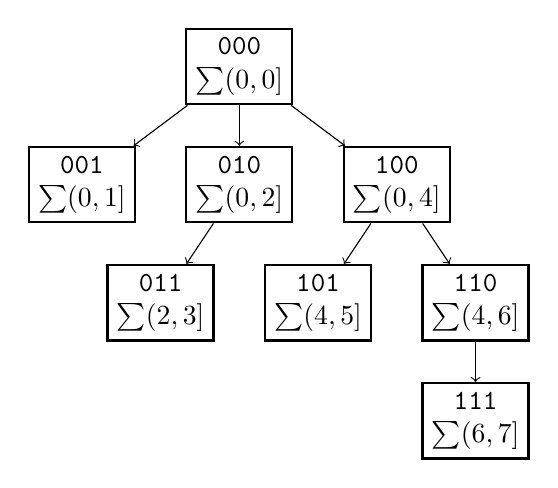
\begin{tikzpicture}
        \node (0) at (0, 0) [draw, thick, align=center] {\texttt{000}\\$\sum(0, 0]$};
        \node (1) at (-2, -1.5) [draw, thick, align=center] {\texttt{001}\\$\sum(0, 1]$};
        \node (2) at (0, -1.5) [draw, thick, align=center] {\texttt{010}\\$\sum(0, 2]$};
        \node (4) at (2, -1.5) [draw, thick, align=center] {\texttt{100}\\$\sum(0, 4]$};
        \node (3) at (-1, -3) [draw, thick, align=center] {\texttt{011}\\$\sum(2, 3]$};
        \node (5) at (1, -3) [draw, thick, align=center] {\texttt{101}\\$\sum(4, 5]$};
        \node (6) at (3, -3) [draw, thick, align=center] {\texttt{110}\\$\sum(4, 6]$};
        \node (7) at (3, -4.5) [draw, thick, align=center] {\texttt{111}\\$\sum(6, 7]$};
        \draw[->] (0) -- (1);
        \draw[->] (0) -- (2);
        \draw[->] (0) -- (4);
        \draw[->] (2) -- (3);
        \draw[->] (4) -- (5);
        \draw[->] (4) -- (6);
        \draw[->] (6) -- (7);
    \end{tikzpicture}
\end{figure}
\vspace{-0.3cm}
Note that the number of elements in the tree is fixed. The tree is implemented such that every child of the root corresponds to a power of two (each sub-tree is then a Fenwick tree itself). This node then contains a prefix sum.
\code{src/datastr/fenwick.cc}



\subsection{Segment tree}

A segment tree is more efficient in calculating sums of intervals than Fenwick trees, and also has more flexibility in the operation that needs to be determined over an interval. Segment trees have two basic operations:
\begin{itemize}
    \item \textsc{sum:} Get the sum of the elements on an interval $[a, b]$. $\mathcal O(\log n)$
    \item \textsc{update:} Update an entry in list that the tree represents. $\mathcal O(\log n)$
\end{itemize}
\vspace{-0.3cm}
\begin{figure}[H]
    \centering
    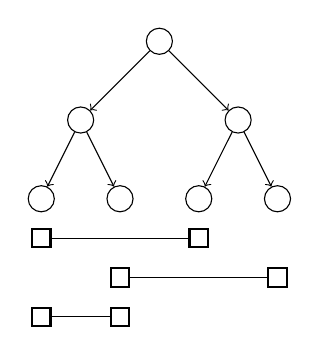
\begin{tikzpicture}[main/.style = {draw, circle, align=center}, node distance=2cm]
        \node[main] (0) at (0, 0) {};
        \node[main] (1) at (-1, -1) {};
        \node[main] (2) at (1, -1) {};
        \node[main] (3) at (-1.5, -2) {};
        \node[main] (4) at (-0.5, -2) {};
        \node[main] (5) at (0.5, -2) {};
        \node[main] (6) at (1.5, -2) {};

        \node (m1) at (-1.5, -2.5) [draw, align=center, thick] {};
        \node (m2) at (0.5, -2.5) [draw, align=center, thick] {};
        \node (m3) at (-0.5, -3) [draw, align=center, thick] {};
        \node (m4) at (1.5, -3) [draw, align=center, thick] {};
        \node (m5) at (-1.5, -3.5) [draw, align=center, thick] {};
        \node (m6) at (-0.5, -3.5) [draw, align=center, thick] {};

        \draw (m1) -- (m2);
        \draw (m3) -- (m4);
        \draw (m5) -- (m6);

        \draw[->] (0) -- (1);
        \draw[->] (0) -- (2);
        \draw[->] (1) -- (3);
        \draw[->] (1) -- (4);
        \draw[->] (2) -- (5);
        \draw[->] (2) -- (6);
    \end{tikzpicture}
\end{figure}
\vspace{-0.3cm}
The implementation uses nodes which store the sum of all of the leaves below it. The start and end points of all of the intervals are considered in the tree.
\code{src/datastr/segment.cc}



\subsection{Sparse table}

A sparse table is similar to a segment tree, but the values of the entries cannot be changed. At creation a table is generated that can then be used to query the minimum of a certain range. The sparse table has two basic operations:
\begin{itemize}
    \item \textsc{build:} Initialization creates the lookup table for a source list. $\mathcal O(n \log n)$
    \item \textsc{query:} Get the minimum value in the list in a range of indices $[l, r)$. $\mathcal O(1)$
\end{itemize}
\begin{figure}[H]
    \centering
    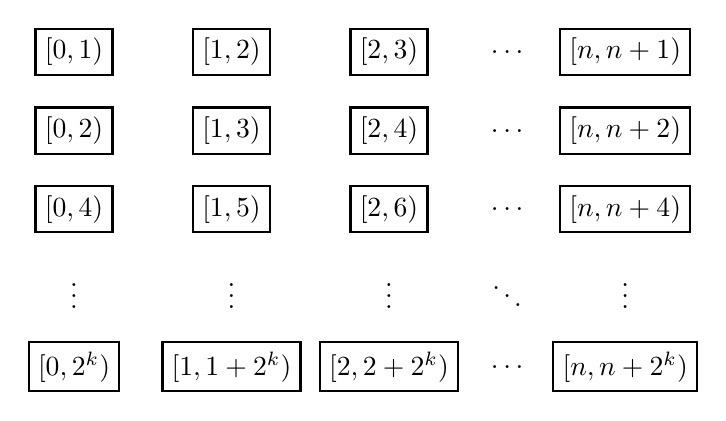
\begin{tikzpicture}
        \node[draw, thick] (A0) at (0, 0) {$[0, 1)$};
        \node[draw, thick] (A1) at (0, -1) {$[0, 2)$};
        \node[draw, thick] (A2) at (0, -2) {$[0, 4)$};
        \node (d) at (0, -3) {$\vdots$};
        \node[draw, thick] (A3) at (0, -4) {$[0, 2^k)$};

        \node[draw, thick] (A0) at (2, 0) {$[1, 2)$};
        \node[draw, thick] (A1) at (2, -1) {$[1, 3)$};
        \node[draw, thick] (A2) at (2, -2) {$[1, 5)$};
        \node (d) at (2, -3) {$\vdots$};
        \node[draw, thick] (A3) at (2, -4) {$[1, 1 + 2^k)$};

        \node[draw, thick] (A0) at (4, 0) {$[2, 3)$};
        \node[draw, thick] (A1) at (4, -1) {$[2, 4)$};
        \node[draw, thick] (A2) at (4, -2) {$[2, 6)$};
        \node (d) at (4, -3) {$\vdots$};
        \node[draw, thick] (A3) at (4, -4) {$[2, 2 + 2^k)$};

        \node (d) at (5.5, 0) {$\dots$};
        \node (d) at (5.5, -1) {$\dots$};
        \node (d) at (5.5, -2) {$\dots$};
        \node (d) at (5.5, -3) {$\ddots$};
        \node (d) at (5.5, -4) {$\dots$};

        \node[draw, thick] (A0) at (7, 0) {$[n, n + 1)$};
        \node[draw, thick] (A1) at (7, -1) {$[n, n + 2)$};
        \node[draw, thick] (A2) at (7, -2) {$[n, n + 4)$};
        \node (d) at (7, -3) {$\vdots$};
        \node[draw, thick] (A3) at (7, -4) {$[n, n + 2^k)$};
    \end{tikzpicture}
\end{figure}
\vspace{-0.3cm}
The implementation calculates the minimum of all intervals $[i, i + 2^k)$ and puts them in a table. Then the minimum of any interval $[\ell, r)$ can be determined by taking the minimum of the largest interval $[\ell, \ell + 2^k)$ that is contained in $[\ell, r)$, and likewise the minimum of the largest interval $[a, r)$. These intervals may overlap, which does not matter in the case of a minimum/maximum.
\code{src/datastr/sparsetable.cc}


\subsection{Interval tree}

An interval tree is used to find all (closed and bounded) intervals containing a point in the tree. The tree supports two basic operations:
\begin{itemize}
    \item \textsc{insert:} Insert an interval into the tree. $\mathcal O(\log n)$
    \item \textsc{search:} Find all $m$ intervals that contain a given point. $\mathcal O(\log n + m)$
\end{itemize}
The tree is implemented as a binary search tree with the left bound of the intervals being the key, and containing annotations about the maximum value in a subtree.
\begin{figure}[H]
    \centering
    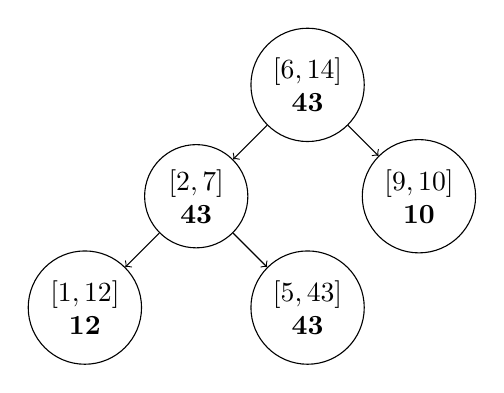
\begin{tikzpicture}[main/.style = {draw, circle, align=center}, node distance=2cm]
        \node[main] (0) {$[6, 14]$\\$\mathbf{43}$};
        \node[main] (1) [below right of=0] {$[9, 10]$\\$\mathbf{10}$};
        \node[main] (2) [below left of=0] {$[2, 7]$\\$\mathbf{43}$};
        \node[main] (3) [below left of=2] {$[1, 12]$\\$\mathbf{12}$};
        \node[main] (4) [below right of=2] {$[5, 43]$\\$\mathbf{43}$};
        \draw[->] (0) -- (1);
        \draw[->] (0) -- (2);
        \draw[->] (2) -- (3);
        \draw[->] (2) -- (4);
    \end{tikzpicture}
\end{figure}
\vspace{-0.3cm}
\code{src/datastr/intervaltree.cc}



\subsection{$k$-d tree}

A $k$-d tree can quickly search and insert points in a multi-dimensional data structure. It supports two basic operations:
\begin{itemize}
    \item \textsc{insert:} Insert a point into the tree. $\mathcal O(k\log n)$
    \item \textsc{search:} Check if the given point is contained in the tree. $\mathcal O(k\log n)$
\end{itemize}
The tree is implemented by having each layer compare a different dimension in a cycle.
\begin{figure}[H]
    \centering
    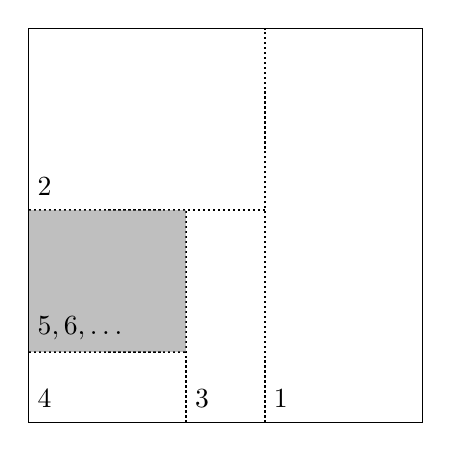
\begin{tikzpicture}
        \draw (0, 0) rectangle (5, 5);
        \draw[densely dotted, thick] (3, 0) -- (3, 5);
        \draw[densely dotted, thick] (0, 2.7) -- (3, 2.7);
        \draw[densely dotted, thick] (2, 0) -- (2, 2.7);
        \draw[densely dotted, thick] (0, 0.9) -- (2, 0.9);
        \fill[fill=gray, opacity=0.5] (0, 2.7) rectangle (2, 0.9);

        \node (0) at (3.2, 0.3) {$1$};
        \node (1) at (0.2, 3) {$2$};
        \node (2) at (2.2, 0.3) {$3$};
        \node (3) at (0.2, 0.3) {$4$};
        \node (4) at (0.65, 1.2) {$5, 6, \dots$};
    \end{tikzpicture}
\end{figure}
\vspace{-0.3cm}
\code{src/datastr/kdtree.cc}





\section{Graphs}

\subsection{Theorems}

\subsubsection{Euler's formula}
For any connected planar graph $(V, E, F)$, which is a graph that can be drawn in $2$-D without intersecting edges, we have
\begin{align*}
    V - E + F = 2.
\end{align*}
Here $V$ is the number of vertices, $E$ the number of edges and $F$ the number of faces (including the outside). For a non-connected planar graph with $C$ connected components, we have
\begin{align*}
    V - E + F = C + 1.
\end{align*}

\subsubsection{Eulerian cycle}
An Eulerian path is a path that uses each edge exactly once. An Eulerian cycle starts and ends in the same vertex. For an undirected connected graph, an Eulerian cycle exists if and only if every vertex has even degree.

A strongly connected directed graph has an Eulerian cycle if and only if all vertices have the same in degree and out degree.

\subsubsection{Eulerian path}
For an undirected connected graph, an Eulerian path exists if and only if there are exactly zero or two vertices with odd degree.

A strongly connected directed graph has an Eulerian path if and only if at most one vertex has in degree one more than out degree, at most one vertex has out degree one more than in degree, and every other vertex has equal in degree and out degree.

\subsubsection{Dirac's/Ore's theorem}
Let $(V, E)$ be a connected graph such that for all $x, y \in V$ with $x \neq y$ we have $d(x) + d(y) \geq |V|$, then $G$ contains a Hamiltonian circuit. The graph $G$ is still Hamiltonian if this only holds for adjacent $x$ and $y$.

\subsubsection{Cayley's theorem}
For $n \geq 1$ there are $n^{n-2}$ tree graphs on $n$ labelled vertices.

\subsubsection{Kőnig's theorem}
In a bipartite graph, the minimum vertex cover has the same size as the maximum matching set.

A vertex cover is a set of vertices such that every edge has at least one vertex that is part of the vertex cover. A matching set is a set of edges such that no vertex is included in more than one edge.

\subsubsection{Max-flow min-cut theorem}
The minimum cut in a flow network is the same as the maximum flow. Min-cut is the minimum total weight of edges to remove such that the source and sink are no longer connected. The max-flow is the maximum flow of some liquid from the source to the sink.

\subsubsection{Maximum independent set}
The maximum independent set of a graph is the maximum size set of vertices that do not share an edge. The complement of the maximum independent set is a minimum vertex cover.

\subsubsection{Petersen graph}
The Petersen graph is often used for counterexamples in graph theory:
\vspace{-0.3cm}
\begin{figure}[H]
    \centering
    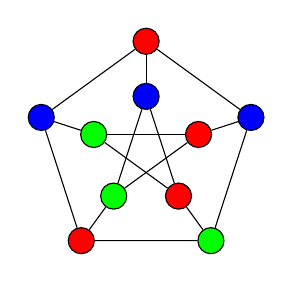
\begin{tikzpicture}[scale=0.7, main/.style = {draw, circle, align=center}, node distance=2cm]
        \node[main, fill=blue] (0) at (0, 1) {};
        \node[main, fill=red] (1) at (0.951, 0.309) {};
        \node[main, fill=red] (2) at (0.588, -0.809) {};
        \node[main, fill=green] (3) at (-0.588, -0.809) {};
        \node[main, fill=green] (4) at (-0.951, 0.309) {};

        \def\rdifft{2}
        \node[main, fill=red] (5) at (0, \rdifft*1) {};
        \node[main, fill=blue] (6) at (\rdifft*0.951, \rdifft*0.309) {};
        \node[main, fill=green] (7) at (\rdifft*0.588, \rdifft*-0.809) {};
        \node[main, fill=red] (8) at (\rdifft*-0.588, \rdifft*-0.809) {};
        \node[main, fill=blue] (9) at (\rdifft*-0.951, \rdifft*0.309) {};
        \draw (0) -- (2);
        \draw (0) -- (3);
        \draw (1) -- (3);
        \draw (1) -- (4);
        \draw (2) -- (4);

        \draw (5) -- (0);
        \draw (6) -- (1);
        \draw (7) -- (2);
        \draw (8) -- (3);
        \draw (9) -- (4);

        \draw (5) -- (6) -- (7) -- (8) -- (9) -- (5);
    \end{tikzpicture}
\end{figure}
\vspace{-0.3cm}



\subsection{Shortest path}

\subsubsection{Dijkstra $\mathcal O(E\log V)$}
The shortest path is found by iteratively picking the shortest edge from a node in the currently reached set to any other node.
\code{src/graph/dijkstra.cc}

\subsubsection{Floyd-Warshall $\mathcal O(V^3)$}
Calculates shortest distances between all nodes by considering a route "via $k$".
\code{src/graph/fw.cc}

\subsubsection{Flood fill reachable nodes $\mathcal O(EM)$}
Only works for graphs with distances in $\{0, 1\}$. Note that the complexity is dependent on $M$, the maximum distance to any node. Only use this if $M$ is low, otherwise use Dijkstra and select nodes based on distance.

This algorithm can be modified to calculate reachable nodes for any graph, but then the maximum distance requirement has to be dropped.
\code{src/graph/floodreach.cc}

\subsubsection{$k$ shortest paths}
A modified version of Dijkstra's algorithm can be used to find the $k$ shortest paths in an undirected graph. Note that this implementation is very slow!
\code{src/graph/kshortest.cc}

\subsubsection{IDA*}
This algorithm is used for finding the shortest path in many AI applications. Suppose we want to find the shortest path from $s$ to $t$. The algorithm uses a heuristic $h: V \to \mathbb R_{\geq 0}$ that has the property
\begin{align*}
    h(v) \leq d(v, t), \quad v \in V.
\end{align*}
It uses a kind of DFS with updating thresholds for further searching.
\code{src/graph/ida.cc}



\subsection{Minimum spanning tree}

When working with a general graph, Prim is likely best. When finding the MST of points (which are all connected by distance) on a 2D surface, Kruskal is likely best.

\subsubsection{Prim $\mathcal O(E\log V)$}
Prim starts at some node and expands the tree by adding the node at the shortest distance from the tree that has not been added yet.
\code{src/graph/prim.cc}

\subsubsection{Kruskal $\mathcal O(E\log V)$}
Kruskal sorts the edges from short to long. And walks through the edges, keeping the vertices in groups using a disjoint-set. If two vertices are already in the same group, edges between them will not be included.
\code{src/graph/kruskal.cc}



\subsection{Topological sort $\mathcal O(V + E)$}

A topological ordering on a directed graph $G = (V, E)$ is an ordering $(v_1, \dots, v_n)$ of the vertices of the graph such that for any $(v_i, v_j) \in E$ we have $i < j$. A topological ordering exists if and only if $G$ does not contain cycles. A topological ordering can be found using DFS.
\code{src/graph/toposort.cc}



\subsection{Cycle finding $\mathcal O(V + E)$}

To check if an undirected graph has a cycle: Use a DSU to find number of connected components $C$ and check if $E + C > V$. To find the cycle, use DFS as below. For directed graphs, remove the marked if-statement below.
\code{src/graph/findcycle.cc}

% \subsubsection{Directed Graph $\mathcal O(V + E)$}
% A cycle in a directed graph can be detected using DFS, in a similar way to topological sort. The implementation detects if there is a "back edge" in the DFS, which means that there is an edge to a node that is currently on the DFS stack.
% \code{src/graph/directedcycle.cc}



\subsection{Strongly connected components $\mathcal O(V + E)$}
A directed graph is strongly connected if there exists a path from every node to every other node (so not just in one direction). In an undirected graph, the connected components can be found with a DSU or BFS/DFS. In directed graphs, Kosaraju's algorithm can be used.
\code{src/graph/kosaraju.cc}


\subsection{Eulerian cycles}

\subsubsection{Existence in an undirected graph $\mathcal O(V + E)$}
An undirected graph contains an Eulerian cycle if and only if it is connected and all vertices have even degrees.
% \code{src/graph/eulerundirected.cc}

\subsubsection{Existence in a directed graph $\mathcal O(V + E)$}
An undirected graph contains an Eulerian cycle if and only if it is strongly connected and all vertices have an equal in and out-degree.
% \code{src/graph/eulerdirected.cc}

\subsubsection{Finding $\mathcal O(E\log E)$}
An Eulerian cycle (if it exists) can be found by using Hierholzer's algorithm. This algorithm first generates some cycle from the starting vertex and then keeps adding cycles at the vertices in this cycle that have unused edges. If an Eulerian cycle exists, it is impossible to get stuck.
\code{src/graph/hierholzer.cc}



\subsection{Max-flow $\mathcal O(E^2V)$ / $\mathcal O(EV^2)$}

The max-flow problem asks for the maximum flow through a directed network (graph) given the capacities of its edges. It can be thought of as a network of water pipes for example.

The problem can be solved using the Edmonds-Karp variant of the Ford-Fulkerson algorithm or Dinic's algorithm.

\subsubsection{Edmonds-Karp algorithm $\mathcal O(E^2V)$}
\code{src/graph/edmonds_karp.cc}

\subsubsection{Dinic's algorithm $\mathcal O(EV^2)$}
If the network is a unit network, meaning every node except $s$ and $t$ has either a unique incoming or a unique outgoing edge, and this unique edge has capacity $1$, then the complexity is reduced to $\mathcal O(E\sqrt V)$.
\code{src/graph/dinic.cc}

\subsubsection{Max-flow min-cut theorem}
Given a network, the capacity of the minimum cut (which has one partition with $s$ and one with $t$) is the same as the maximum flow in the network.



\subsection{Maximum bipartite matching $\mathcal O(E\sqrt V)$}

The maximum matching (maximum number of vertex pairs that have an edge between them) in a bipartite graph with parts $A$ and $B$ can be found using Dinic's algorithm (see above), by setting all capacities to 1.
\vspace{-0.2cm}
\begin{figure}[H]
    \centering
    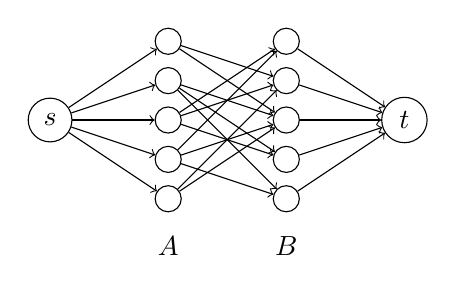
\begin{tikzpicture}[main/.style = {draw, circle}, node distance=1cm]
        \node[main] at (0, 0) (0) {$s$};
        
        \node[main] at (1.5, -1) (1) {};
        \node[main] at (1.5, -0.5) (2) {};
        \node[main] at (1.5, 0) (3) {};
        \node[main] at (1.5, 0.5) (4) {};
        \node[main] at (1.5, 1) (5) {};
        \node[] at (1.5, -1.6) (A) {$A$};

        \node[main] at (3, -1) (6) {};
        \node[main] at (3, -0.5) (7) {};
        \node[main] at (3, 0) (8) {};
        \node[main] at (3, 0.5) (9) {};
        \node[main] at (3, 1) (10) {};
        \node[] at (3, -1.6) (B) {$B$};

        \node[main] at (4.5, 0) (11) {$t$};
        
        \draw[->] (0) -- (1);
        \draw[->] (0) -- (2);
        \draw[->] (0) -- (3);
        \draw[->] (0) -- (4);
        \draw[->] (0) -- (5);

        \draw[->] (1) -- (8);
        \draw[->] (1) -- (9);
        \draw[->] (2) -- (6);
        \draw[->] (2) -- (8);
        \draw[->] (2) -- (10);
        \draw[->] (3) -- (7);
        \draw[->] (3) -- (9);
        \draw[->] (3) -- (10);
        \draw[->] (4) -- (6);
        \draw[->] (4) -- (7);
        \draw[->] (4) -- (8);
        \draw[->] (5) -- (8);
        \draw[->] (5) -- (9);

        \draw[->] (6) -- (11);
        \draw[->] (7) -- (11);
        \draw[->] (8) -- (11);
        \draw[->] (9) -- (11);
        \draw[->] (10) -- (11);
    \end{tikzpicture}
\end{figure}
\vspace{-0.2cm}



\subsection{Assignment problem $\mathcal O(V^3)$}

The Hungarian algorithm solves the assignment problem: Given a complete bipartite graph with parts $S$ and $T$, and a cost $c_{ij}$ for each $i \in S$ and $j \in T$, find a perfect matching (all vertices are in a match) with minimal summed cost.
\code{src/graph/hungarian.cc}



\subsection{Maximum independent set of a tree $\mathcal O(E)$}

A maximum independent set in a graph is a set of vertices of maximum size such that no two vertices share an edge. In a tree, the maximum independent set can be determined using DFS, by determining the maximum independent set with both the current node included and not included.
\code{src/graph/maxindep.cc}



\subsection{Graph coloring}

A coloring of a graph is an assignment of colors to the vertices such that two vertices connected by an edge have a different color. The problem is generally NP-hard.

\subsubsection{Chromatic polynomial}
The chromatic polynomial represents the number of ways a graph can be colored given a maximum number of colors $x$. Below are some common graph types:
\begin{table}[H]
    \centering
    \begin{tabular}{|l|c|}
        \hline
        Graph & $\mathcal P(x)$ \\
        \hline
        Complete $K_n$ & $x(x - 1)(x - 2)\dots(x - (n - 1))$ \\
        Edgeless $\overline K_n$ & $x^n$ \\
        Tree with $n$ vertices & $x(x - 1)^{n - 1}$ \\
        Cycle $C_n$ & $(x - 1)^n + (-1)^n(x - 1)$ \\
        Path $P_n$ & $x(x - 1)^{n - 1}$ \\
        Star $S_n$ & $x(x - 1)^{n - 1}$ \\
        Ladder $P_2 \times P_n$ & $x(x - 1)(x^2 - 3x + 3)^{n - 1}$ \\
        \hline
    \end{tabular}
    \label{tab:chromatic}
\end{table}

\subsubsection{Chromatic number}
The chromatic number $\chi(G)$ is the minimum number of colors needed to color the graph $G$, it has the following properties:
\begin{align*}
    \chi(G) &:= \min\{k \in \mathbb N \mid \mathcal P(k) > 0\}, \\
    \chi(G)(\xi(G) - 1) &\leq 2|E|, \\
    \chi(G) &\geq \omega(G), \\
    \chi(G) &\leq 1 + \max_{v\in V} d(v),
\end{align*}
where $\omega(G)$ is the size of the size of the largest clique (complete subgraph).

\subsubsection{2-coloring $\mathcal O(V + E)$}
A graph can be colored with 2 colors if it is bipartite. This can be found out using BFS.
\code{src/graph/bipartite.cc}

% \subsubsection{Greedy coloring $\mathcal O(V + E)$}
% Greedy algorithm to find some coloring of a graph, by iterating over the vertices in some order and picking the first color that is different from the colors of its neighbours.
% \code{src/graph/greedycoloring.cc}





\section{Search algorithms}
The following are in the \texttt{C++} STL:
\begin{itemize}
    \item \texttt{find(begin, end, val)}: Returns iterator to found element (linear search).
    \item \texttt{find\_if(begin, end, pred)}: Returns iterator for element that returns \texttt{true} for given predicate. For example \texttt{find\_if(all(vec), [] (ll v) \{ return v \% 2 == 0 \})} returns the first even element.
\end{itemize}

\subsection{Binary search $\mathcal O(\log(max - min))$}

Find the lowest number $x$ in an interval $[s, t]$ such that $f(x)$ holds. Assumes that for any $x \in [s, t]$ with $f(x)$ true, $f(y)$ holds for all $y \geq x$.

Binary search on a sorted vector in \texttt{C++} can be done using \texttt{binary\_search} (will check if element exists).
\code{src/search/binary.cc}

\subsection{Ternary search $\mathcal O(\log(max - min))$}

Finds the maximum $M$ of a function that is monotonically increasing for values lower than $M$ and monotonically decreasing for values higher than $M$. This can be used as a replacement for determining the point where the derivative is zero, for example in the case of a parabola.
\code{src/search/ternary.cc}

\subsection{Interpolation search $\mathcal O(\log(\log n))$}

This algorithm is faster than binary search if the data in a list is uniformly distributed (otherwise it is $\mathcal O(\log n)$). The algorithm guesses a position of the element based on the current lower and upper bounds.
\code{src/search/interpolation.cc}





\section{Sort algorithms}

A version of Quicksort (combined with linear sort) is implemented in \texttt{C++}, use \texttt{sort(all(list), lt)}. Or use \texttt{stable\_sort(all(list), lt)} for stable sorting.

\subsection{Quicksort $\mathcal O(n\log n)$}

In case more complicated mechanics need to be implemented, the following template can be used:
\code{src/sort/qs.cc}

\subsection{Counting sort $\mathcal O(max - min + n)$}

Can be used when the range of values in the list is very small, searches roughly in linear time. Most of the time, Quicksort (STL) is better.
\code{src/sort/count.cc}

\subsection{Random sort $\mathcal O(n\log n)$}

\code{src/sort/random.cc}

\subsection{Count inversions $\mathcal O(n\log n)$}

This algorithm counts the number of inversions in a list using merge-sort. An inversion is a pair $(x_i, x_j)$ in a list $(x_1, x_2, \dots, x_n)$ where $i < j$ and $x_i > x_j$.
\code{src/sort/inversions.cc}





\section{String algorithms}

In \texttt{C++} some built-in functions on strings are:
\begin{itemize}
    \item \texttt{s.find(it, pos = 0)}, does not use KMP. $\mathcal O(mn)$
    \item \texttt{s.substr(start, end = SIZE\_MAX)}. $\mathcal O(end - start)$
\end{itemize}

\subsection{Knuth-Morris-Pratt $\mathcal O(S + P)$}

This algorithm determines the position of a pattern $P = p_1p_2\dots p_m$ in a string $S = s_1s_2\dots s_n$, where $n > m$. It does this by first preprocessing the pattern and then matching the string in constant time. In case there are multiple strings where the same pattern needs to be matched, the preprocessing step only has to be done once.
\code{src/string/kmp.cc}



\subsection{Aho-Corasick $\mathcal O(\sum_i S_i + \sum_i P_i + M)$}

Like KMP, it is used for finding patterns in strings. However, all patterns are processed in a batch, which is more cost-efficient than matching using KMP for every pattern. It constructs an automaton on 3 steps: Construct a trie, add blue edges, and add green edges. The blue edges point to the longest strict suffix of the current word in the trie. The green edges point to the longest \textit{accepted} suffix in the tree (may not exist). The complexity is the sum of the total string length, total pattern length, and the number of matches. The number of matches can be removed from the complexity if only the longest suffix is returned for each index.
\vspace{-0.3cm}
\begin{figure}[H]
    \centering
    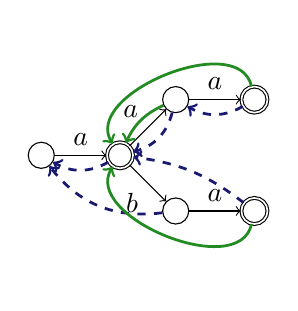
\begin{tikzpicture}[main/.style = {draw, circle}, node distance=1cm]
        \node[main] (0) {};
        \node[main,double] (1) [right of=0] {};
        \node[main] (2) [above right of=1] {};
        \node[main] (3) [below right of=1] {};
        \node[main,double] (4) [right of=2] {};
        \node[main,double] (5) [right of=3] {};
        \draw[->] (0) -- node[midway,above] {$a$} (1);
        \draw[->] (1) -- node[midway,above left] {$a$} (2);
        \draw[->] (1) -- node[midway,below left] {$b$} (3);
        \draw[->] (2) -- node[midway,above] {$a$} (4);
        \draw[->] (3) -- node[midway,above] {$a$} (5);
        \draw[->,dashed,color=MidnightBlue,line width=1pt] (1) to[bend left] (0);
        \draw[->,dashed,color=MidnightBlue,line width=1pt] (2) to[bend left] (1);
        \draw[->,dashed,color=MidnightBlue,line width=1pt] (3) to[bend left] (0);
        \draw[->,dashed,color=MidnightBlue,line width=1pt] (5) to[bend angle=15,bend right] (1);
        \draw[->,dashed,color=MidnightBlue,line width=1pt] (4) to[bend left] (2);
        \draw[->,color=ForestGreen,line width=1pt] (5) to[bend angle=100,bend left] (1);
        \draw[->,color=ForestGreen,line width=1pt] (2) to[bend angle=20,bend right] (1);
        \draw[->,color=ForestGreen,line width=1pt] (4) to[bend angle=100,bend right] (1);
    \end{tikzpicture}
\end{figure}
\vspace{-0.3cm}
\code{src/string/ahocorasick.cc}



\subsection{Edit distance $\mathcal O(S_1S_2)$}

Given two strings, the edit distance is the minimum amount of operations needed to transform one string into another, with the operations insert character, remove character, replace character. The implementation uses DP on first $m$ characters of $S_1$ and $n$ characters of $S_2$.
\code{src/string/edit.cc}



% \subsection{Shortest prefix $\mathcal O(\sum_i P_i)$}

% \code{src/string/prefix.cc}



\subsection{Longest common subsequence $\mathcal O(S_1S_2)$}

\code{src/string/subseq.cc}





\section{Miscellaneous}

\subsection{Knapsack problem $\mathcal O(Wn)$}

\code{src/misc/knapsack.cc}



\subsection{Hashing}

Default \texttt{C++} structures often support hashing by the default, such as \texttt{string}, \texttt{long long}, etc. These are automatically used in \texttt{unordered\_map} and \texttt{unordered\_set} to give $\mathcal O(1)$ lookup times.

\subsubsection{Rolling hash function}
You can make it so that the hash of an object can be determined based on its individual elements (such as in a vector). For example a string $s_1s_2\dots s_n$ can be hashed with
\begin{align*}
    H(s_1s_2\dots s_n) = \sum_{k=1}^n s_kp^{k-1}\mod M,
\end{align*}
for some small prime $p$ and large prime $M$ (see "Useful numbers"). This then gives the relations
\begin{align*}
    H(s_1s_2\dots s_ns_{n+1}) &\equiv H(s_1s_2\dots s_n) + s_{n+1}p^{n}, \\
    H(s_0s_1\dots s_n) &\equiv s_0 + pH(s_1s_2\dots s_n), \\
    H(s_2s_3\dots s_n) &\equiv p^{-1}\left(H(s_1s_2\dots s_n) - s_1\right), \\
    H(s_1s_2 \dots s_{n-1}) &\equiv H(s_1s_2\dots s_n) - s_{n}p^{n - 1}.
\end{align*}
\code{src/misc/rollinghash.cc}

\subsubsection{Custom hash function}
C++ doesn't have hash functions for vectors and pairs, add them like this:
\code{src/misc/hash.cc}



% \subsection{Parser}

% \code{src/misc/parser.cc}



\subsection{Gray code}
Gray code is a way of ordering binary numbers, such that two consecutive numbers differ in exactly one bit. Iterating over binary numbers in this way can be used for optimizations when using bitmasks.

\code{src/misc/gray.cc}
\code{src/misc/grayinv.cc}



\subsection{Interval cover $\mathcal O(n\log n)$}

\code{src/misc/intervalcover.cc}



\subsection{Stable matching problem $\mathcal O(n^2)$}

The stable matching problem is to find a stable matching given two lists of objects of size $n$. Each object in both lists has a priority list for the objects in the other list. A matching is \textit{un}stable if both of the following occur:
\begin{enumerate}
    \item There is an element $A$ of the first list, and an element $B$ of the second list, such that $A$ prefers $B$ over the current assignment, and
    \item $B$ prefers $A$ over its assigned element.
\end{enumerate}
A stable matching can always be found, and can be found using the Gale-Shapley algorithm. The algorithm finds the stable matching that is best for the first group and worst for the second group.
\code{src/misc/stablematching.cc}



\subsection{Subset sum problem $\mathcal O(n(max - min))$}

The subset sum problem is to determine if there is a subset $\tilde X$ of a multiset of integers $X$, such that $\sum \tilde X = T$. The problem is NP-hard when the possible sums are unbounded. It can be solved by keeping track of all possible subset sums of the first $k$ elements. To find the elements that make up the sum, a directed graph can be used with vertices $(k, t)$, which indicates that the first $k$ elements contain a subset sum of $t$. Then there are edges from $(k, t)$ to $(k + 1, t)$ and $(k + 1, t + x_{k + 1})$. A path from $(0, 0)$ to $(n, T)$ can be found with DFS/BFS.
\code{src/misc/subsetsum.cc}



\subsection{Longest increasing subsequence}

\code{src/misc/longestincreasing.cc}



\subsection{Approximate bounds}

Below is a table of approximate upper bounds for $n$ given different algorithm complexities. Keep in mind that constants may also be high, but generally this is not important.

\begin{table}[H]
    \centering
    \begin{tabular}{ll}
        \hline
        \textbf{Complexity} \hspace{2em} & \textbf{Bound} \\
        \hline
        $\mathcal O(n!)$ & $n \leq 10$ \\
        $\mathcal O(2^n)$ & $n \leq 20$ \\
        $\mathcal O(n^3)$ & $n \leq 500$ \\
        $\mathcal O(n^2\log n)$ & $n \leq 10^3$ \\
        $\mathcal O(n^2)$ & $n \leq 5\cdot 10^3$ \\
        $\mathcal O(n\sqrt n)$ & $n \leq 10^5$ \\
        $\mathcal O(n\log^2 n)$ & $n \leq 10^5$ \\
        $\mathcal O(n\log n)$ & $n \leq 10^6$ \\
        $\mathcal O(n)$ & $n \leq 10^8$ \\
        $\mathcal O(\sqrt n)$ & $n \leq 10^{15}$ \\
        $\mathcal O(\log n)$ & $n \leq 10^{18}$ \\
        \hline
    \end{tabular}
    \label{tab:modinv}
\end{table}





\section{Pre-competition checklist}

\subsubsection{Before competition}
\begin{itemize}
    \item What time do we need to wake up?
    \item Make sure to be on time for test session and competition!
    \item Can we take snacks with use? Pepsels, Oreo's, etc. ;)
    \item Remember to bring a bottle of water!
    \item Do we know the amount of problems there will be?
    \item Discuss reading order/strategy.
    \item Hand in reference document, keyboard and mouse at registration.
    \item How many copies of this document can we use?
    \item Which IDE is used? Check useful shortcuts. VSCode?
    \item Which languages are supported? C++? Python?
\end{itemize}

\subsubsection{Test session}
\begin{itemize}
    \item Which feedback is given on incorrect result? Check for \textsf{no output}, \textsf{wrong answer}, \textsf{timelimit}, \textsf{runtime error}, \textsf{output limit}, \textsf{memory limit}, \textsf{compiler error}.
    \item Check judging features:
    \begin{itemize}
        \item Is \texttt{cerr} considered as output?
        \item Difference in time with more/less correct results?
        \item Still correct with compiler warnings?
        \item Still correct without \texttt{return 0;}?
        \item Still correct with \texttt{exit(0)}?
        \item Still correct with memory leaks?
    \end{itemize}
    \item Which \texttt{C++} version is used? Optimization level?
\end{itemize}

\subsubsection{Pink elephant}

\begin{center}
    \begin{figure}[H]
        \centering
        
\includegraphics[height=120pt]{pink_elephant.png}
        \label{fig:pink_elephant}
        \vspace{-3em}
    \end{figure}
\end{center}
